\documentclass{article}

\usepackage{arxiv}
\usepackage[utf8]{inputenc}
\usepackage[T1]{fontenc}
\usepackage{hyperref}
\usepackage{url}
\usepackage{booktabs}
\usepackage{tabularx}
\usepackage{array}
\usepackage{amsmath}
\usepackage{amsfonts}
\usepackage{microtype}
\usepackage{graphicx}
\usepackage{tikz}
\usetikzlibrary{arrows.meta,positioning,shapes.geometric}
\usepackage{natbib}
\usepackage{enumitem}
\usepackage{xcolor}

\renewcommand{\headeright}{Technical Report}
\renewcommand{\undertitle}{Candidate Project Report}
\renewcommand{\shorttitle}{Safety-Oriented Execution Algorithm Service}

\hypersetup{
  pdftitle={A Safety-Oriented Execution Algorithm Service for Binance USD-M BTCUSDT},
  pdfsubject={Calais quantitative development candidate project},
  pdfauthor={Haoran Wu},
  pdfkeywords={execution algorithm, TWAP, chase order, Binance futures, deterministic simulator, order state machine}
}

\title{A Safety-Oriented Execution Algorithm Service for Binance USD-M BTCUSDT}

\author{
  Haoran Wu \\
  Calais Quantitative Development Candidate Project \\
  \texttt{calais-execution-algorithm}
}

\date{June 2026}

\newcommand{\code}[1]{\texttt{#1}}
\newcommand{\status}[1]{\textsc{#1}}
\newcommand{\yes}{\textsc{covered}}
\newcommand{\partialstatus}{\textsc{partial}}
\newcommand{\gap}{\textsc{gap}}

\begin{document}
\maketitle

\begin{abstract}
This report describes a compact execution algorithm service for Binance USD-M Futures BTCUSDT Perpetual. The service accepts a final target position, a permitted active execution price range, a target duration, and either a Chase or TWAP execution mode. The design priority is small-but-correct execution behavior rather than broad venue coverage: one symbol, one exchange family, one-way mode, deterministic simulator coverage, and a credential-gated Binance Testnet path. The core safety argument is an exposure invariant that accounts for confirmed fills, live open quantity, pending submits, pending cancels, unknown create outcomes, and proposed child quantity before any new order can be submitted. Deterministic simulator runs cover races that Testnet cannot reliably force, including fill-after-cancel and ambiguous create-timeout reconciliation. Accepted sanitized Binance Testnet artifacts are included for both Chase and TWAP; they preserve order/trade evidence while redacting account balance and position updates. The report itself uses the requested arxiv-style template \citep{arxiv-style}.
\end{abstract}

\keywords{execution algorithm \and order state machine \and overfill prevention \and deterministic simulator \and TWAP \and Chase order}


\section{Introduction}

The project brief asks for a Python execution algorithm for Binance USD-M Futures BTCUSDT Perpetual. The algorithm receives a final account target position, a price interval, a target duration, and an execution algorithm. The most important interpretation is that \code{target\_position} is not an order quantity. The system first reads the current position and computes:

\begin{equation}
  required\_trade\_quantity = target\_position - current\_position.
\end{equation}

A negative-to-positive target therefore requires trading through zero. For example, moving from \(-0.003\) BTC to \(+0.005\) BTC requires buying \(0.008\) BTC, not \(0.005\) BTC. This rule is intentionally placed at execution creation, before algorithm selection, so Chase and TWAP share the same target-position semantics.

The second important interpretation is that price, time, and quantity cannot all be guaranteed across every market path. If a buy price range ends at an upper bound, the implementation cannot legally force a fill above that bound. If the market never becomes executable within the interval, a correct result may be partial or fully unfilled. The report therefore evaluates the project by whether the system reports actual outcome and preserves safety, not whether every run reaches 100 percent completion.

The implementation follows a ``small and correct'' strategy. It avoids multi-asset routing, durable production recovery, and mainnet automation. In exchange, the core order lifecycle is explicit, deterministic tests cover abnormal event ordering, and every child submit passes through the same exposure gate. The central design objective is not guaranteed completion. Price, time, and quantity cannot all be guaranteed under every market path. The objective is instead to make the outcome \textbf{correct, bounded, auditable, and explainable}: never knowingly overfill, never double-count a fill, never retry an ambiguous create with a fresh client order ID before reconciliation, and never report completion when price or exchange rules make completion illegal.

\begin{table}[t]
\caption{Submission status on the final report branch.}
\label{tab:submission-status}
\centering
\small
\begin{tabularx}{\linewidth}{>{\raggedright\arraybackslash}p{0.27\linewidth} X}
\toprule
Area & Status \\
\midrule
Core implementation & FastAPI service, execution engine, Chase, TWAP, simulator, Binance USD-M adapter, structured artifacts, and verification scripts are implemented. \\
Deterministic safety evidence & Simulator artifacts cover normal Chase, TWAP schedule, cancel/fill race, create-timeout reconciliation, duplicate events, stale data, price bounds, dust, and cross-zero target handling. \\
Accepted Binance Testnet evidence & Sanitized Chase and TWAP bundles contain non-empty Binance exchange order IDs, client order IDs, private stream events, reconciliation outputs, and terminal summaries. \\
Rejected connectivity artifacts & Older insufficient-margin Testnet attempts are retained only as connectivity/error evidence and are not counted as accepted order-lifecycle proof. \\
Submission controls & Mainnet mutation is hard-disabled by default; Testnet order sends require credentials and an explicit confirmation flag. \\
\bottomrule
\end{tabularx}
\end{table}

The scoring rubric makes this emphasis natural. Execution correctness and edge cases dominate the score, while report writing is a smaller but important communication channel. The report is therefore structured as a correctness defense. It starts with requirements and ownership boundaries, then spends most of its space on state, safety invariants, failure cases, and evidence. The goal is to make the implementation easy to challenge in an interview: each important claim should point to a module boundary, invariant, test, artifact, or limitation.

\begin{table}[t]
\caption{How the report maps to the visible scoring categories.}
\label{tab:scoring}
\centering
\small
\begin{tabularx}{\linewidth}{>{\raggedright\arraybackslash}p{0.28\linewidth} X}
\toprule
Scoring area & Report emphasis \\
\midrule
Execution correctness & Target position, Decimal math, price bounds, exposure invariant, create-timeout handling. \\
Edge cases and state & Parent and child state machines, cancel/fill race, duplicate events, stale streams, deadline behavior. \\
Testing quality & Deterministic simulator, T1-T10 matrix, raw artifacts, repeatable verification commands. \\
Algorithm design & Chase repricing policy and TWAP absolute schedule with carry-forward deficit. \\
Architecture and communication & Clear ownership boundaries, limitations, AI disclosure, and sanitized Testnet evidence status. \\
\bottomrule
\end{tabularx}
\end{table}

\begin{table}[t]
\caption{Compact requirement coverage. More detailed edge-case and test mappings are in the appendix.}
\label{tab:coverage}
\centering
\small
\begin{tabularx}{\linewidth}{>{\raggedright\arraybackslash}p{0.30\linewidth} X}
\toprule
Requirement area & Evidence or note \\
\midrule
Target-position semantics & Engine computes net delta from current position; no-action and cross-zero cases are tested. \\
Chase and TWAP & Chase passive repricing and TWAP absolute schedule are implemented as narrow algorithm helpers. \\
Price bounds and Decimal math & Decimal-string API fields, Decimal internal math, side-aware rounding, tick/step/min checks. \\
State machines and overfill safety & Parent and child states are monotonic; submit path enforces the exposure invariant. \\
Deterministic simulator & Simulator covers partial fill, cancel/fill race, post-only rejection, create timeout, duplicate/lower fills, stale data, and stream disconnect. \\
Binance Testnet integration code & Adapter and runner implement symbol rules, REST mutation, exact lookup, user streams, and evidence artifacts. \\
Accepted Binance Testnet Chase/TWAP evidence & Accepted sanitized Chase and TWAP artifacts are included with non-empty exchange order IDs. \\
Final reporting and AI disclosure & This LaTeX report and \code{AI\_USAGE.md} document decisions, evidence, and verification. \\
\bottomrule
\end{tabularx}
\end{table}


\section{Architecture and Ownership Boundaries}

The architecture is organized around one rule: the engine owns trading correctness. API and runtime code supervise execution, algorithms compute narrow decisions, and exchange adapters normalize venue behavior. They do not independently mutate exposure.

\begin{figure}[t]
\centering
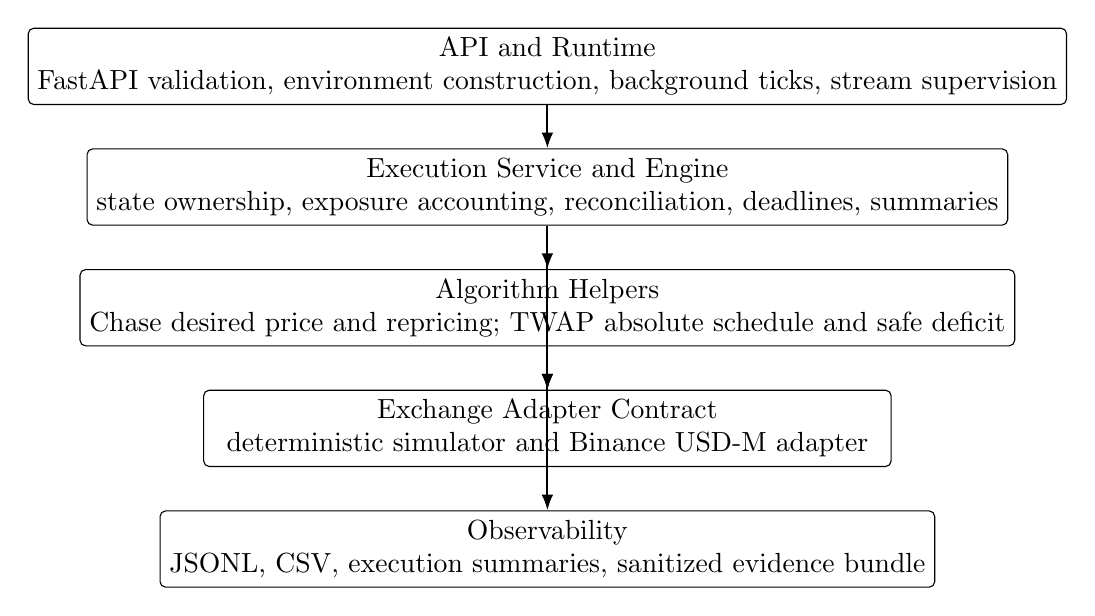
\begin{tikzpicture}[
  node distance=0.55cm,
  box/.style={draw, rounded corners=2pt, align=center, minimum width=0.72\linewidth, minimum height=0.72cm},
  arrow/.style={-{Latex[length=2mm]}, thick}
]
\node[box] (api) {API and Runtime\\FastAPI validation, environment construction, background ticks, stream supervision};
\node[box, below=of api] (service) {Execution Service and Engine\\state ownership, exposure accounting, reconciliation, deadlines, summaries};
\node[box, below=of service] (algo) {Algorithm Helpers\\Chase desired price and repricing; TWAP absolute schedule and safe deficit};
\node[box, below=of algo] (exchange) {Exchange Adapter Contract\\deterministic simulator and Binance USD-M adapter};
\node[box, below=of exchange] (obs) {Observability\\JSONL, CSV, execution summaries, sanitized evidence bundle};
\draw[arrow] (api) -- (service);
\draw[arrow] (service) -- (algo);
\draw[arrow] (algo) -- (exchange);
\draw[arrow] (service) -- (exchange);
\draw[arrow] (service) -- (obs);
\end{tikzpicture}
\caption{Layered ownership. The algorithm layer proposes; the engine decides whether the proposed child order is safe.}
\label{fig:architecture}
\end{figure}

\textbf{Design rule.} Algorithms propose a price, schedule quantity, or reprice decision; the engine decides whether the resulting child order is safe to submit. This rule keeps the most dangerous responsibilities--filled quantity, live exposure, pending cancel quantity, unknown create outcomes, and terminal state--inside one component instead of spreading them across runtime callbacks and algorithm helpers.

\code{ExecutionRuntime} is the API-facing supervisor. It builds the correct environment, rejects concurrent active executions for the same environment and symbol, advances nonterminal executions, supervises market and private streams for Binance-like adapters, renews listen keys, and reconciles after stream events or disconnects.

\code{ExecutionService} is deliberately thin. It delegates execution lifecycle to \code{ExecutionEngine}, which owns parent execution state, child order state, exposure buckets, fill accounting, cancel flow, create-timeout handling, deadline behavior, and terminal summaries. This boundary keeps correctness checks in one place.

\code{Chase} and \code{TWAP} helpers do not submit orders. Chase computes the passive desired price and whether repricing is due. TWAP computes schedule progress and deficit. Both route through the engine's submit path, so price checks, exposure checks, Decimal normalization, and unknown-order reservations remain common.

The concurrency model is intentionally single-process. The runtime rejects a second active execution for the same environment and symbol, and the engine serializes mutations on each execution record so \code{run\_once}, manual cancel, stream-event application, and reconciliation do not race each other inside the process. This does not claim production-grade distributed ownership; it gives the assignment a clear correctness boundary that can be tested deterministically.

\code{ExchangeAdapter} gives the simulator and Binance adapter the same narrow contract: symbol rules, position, best bid/ask, submit, cancel, exact order lookup, stream events, reconciliation, and stream health. This is important because deterministic simulator tests exercise the same engine logic used by the Binance Testnet runner. The simulator is therefore a programmable venue for forced races, not a separate happy-path mock.


\section{Lifecycle and State Machines}

The parent execution lifecycle is monotonic. Terminal executions do not return to \status{RUNNING}. The engine serializes operations per execution so API requests, background ticks, stream events, manual cancel, and reconciliation cannot concurrently mutate the same execution record.

\begin{figure}[t]
\centering
\small
\begin{tabularx}{\linewidth}{>{\raggedright\arraybackslash}p{0.18\linewidth} >{\raggedright\arraybackslash}p{0.28\linewidth} X}
\toprule
Phase & Allowed next phase & Purpose \\
\midrule
\status{CREATED} & \status{VALIDATING} & Request accepted and domain objects built. \\
\status{VALIDATING} & \status{RUNNING} or terminal & Position, symbol rules, bounds, duration, and dust checks. \\
\status{RUNNING} & \status{CANCELLING} or terminal & Submit, cancel, reconcile, deadline, and fill processing. \\
\status{CANCELLING} & terminal & Stop active exposure, reconcile, then summarize. \\
Terminal & none & \status{COMPLETED}, \status{PARTIALLY COMPLETED}, \status{EXPIRED}, \status{CANCELLED}, or \status{FAILED}. \\
\bottomrule
\end{tabularx}
\caption{Parent execution state transition table. Terminal states are one-way.}
\label{fig:execution-state}
\end{figure}

\begin{figure}[t]
\centering
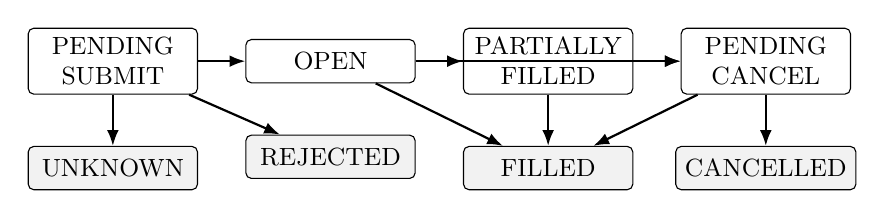
\begin{tikzpicture}[
  node distance=0.48cm and 0.6cm,
  state/.style={draw, rounded corners=2pt, align=center, minimum width=2.15cm, minimum height=0.55cm, font=\small},
  terminal/.style={state, fill=gray!10},
  arrow/.style={-{Latex[length=2mm]}, thick}
]
\node[state] (pending) {PENDING\\SUBMIT};
\node[state, right=of pending] (open) {OPEN};
\node[state, right=of open] (partial) {PARTIALLY\\FILLED};
\node[state, right=of partial] (pcancel) {PENDING\\CANCEL};
\node[terminal, below=0.65cm of pending] (unknown) {UNKNOWN};
\node[terminal, below=0.65cm of open] (rejected) {REJECTED};
\node[terminal, below=0.65cm of partial] (filled) {FILLED};
\node[terminal, below=0.65cm of pcancel] (cancelled) {CANCELLED};
\draw[arrow] (pending) -- (open);
\draw[arrow] (pending) -- (unknown);
\draw[arrow] (pending) -- (rejected);
\draw[arrow] (open) -- (partial);
\draw[arrow] (open) -- (pcancel);
\draw[arrow] (open) -- (filled);
\draw[arrow] (partial) -- (pcancel);
\draw[arrow] (partial) -- (filled);
\draw[arrow] (pcancel) -- (cancelled);
\draw[arrow] (pcancel) -- (filled);
\end{tikzpicture}
\caption{Child order states. \status{UNKNOWN} is a reserved-exposure state, not a harmless error.}
\label{fig:child-state}
\end{figure}

The child state machine is designed for disagreement between REST responses and user-stream events. A fill can arrive after a cancel request. A create request can time out while the exchange still accepts the order. A REST snapshot can be older than a private stream event. The engine therefore treats cumulative fills as monotonic, keeps pending-cancel and unknown-create exposure reserved, and uses exact client-order lookup to repair ambiguous create outcomes.

\textbf{Auditability.} Parent execution IDs, internal child order IDs, and Binance client order IDs are intentionally related. A parent execution such as \code{exec\_3168600ee25b4193} produces client order IDs with a short deterministic prefix such as \code{ce\_3168600ee25b\_1}. This makes logs, child-order CSVs, fill CSVs, reconciliation rows, and Binance order evidence joinable without relying on timestamps alone. It also scopes reconciliation to the execution under review; broad prefix scans can help diagnostics, but exact client-order lookup is the proof used for ambiguous create outcomes.


\section{Core Safety Invariant}

The central correctness claim is the submit gate:

\begin{equation}
\begin{split}
&confirmed\_filled + live\_open + pending\_submit \\
&+ pending\_cancel + unknown\_order + new\_child\_quantity \\
&\le normalized\_target\_trade\_quantity.
\end{split}
\label{eq:invariant}
\end{equation}

This is stronger than recomputing a simple remaining quantity. \code{confirmed\_filled} is parent-level cumulative filled quantity. \code{live\_open} can still trade at the venue. \code{pending\_submit} protects the interval between local intent and exchange response. \code{pending\_cancel} protects the period where a cancel request has been sent but fills can still arrive. \code{unknown\_order} protects ambiguous create outcomes. \code{new\_child\_quantity} is the proposed order.

The two most important buckets are \code{pending\_cancel} and \code{unknown\_order}. If the system releases \code{pending\_cancel} too early, it can submit a replacement while the old order is still fillable. If it releases \code{unknown\_order} after a create timeout, it can retry with a fresh client order ID even though the original order may be live. Both cases can create predictable overfill. Equation~\ref{eq:invariant} prevents this by reserving exposure until reconciliation proves it is gone.

Other invariants support this gate:

\begin{itemize}[leftmargin=1.2em]
  \item Parent confirmed filled quantity is monotonic.
  \item Per-child cumulative filled quantity is monotonic.
  \item Duplicate trade or event messages cannot increase parent fill twice.
  \item A timed-out create remains \status{UNKNOWN} until exact \code{origClientOrderId} reconciliation.
  \item No aggressive child order may violate the configured price bound.
  \item Terminal execution state cannot return to \status{RUNNING}.
\end{itemize}


\section{Chase Design}

Chase uses passive limit orders at the current best queue price: buy orders at best bid and sell orders at best ask. Passive orders are post-only when the venue supports it. Repricing requires both a price movement threshold and a minimum interval:

\begin{equation}
  reprice\_difference\_bps =
  \left|\frac{desired\_price}{active\_order\_price} - 1\right| \times 10000.
\end{equation}

The default repricing mode is \code{ADVERSE\_ONLY}. A buy order reprices upward when the best bid moves up enough; a sell order reprices downward when the best ask moves down enough. This default is deliberately conservative. It avoids unnecessary cancels when the existing order is already passive at a more favorable price and reduces cancel storm risk. \code{TWO\_SIDED} is still available for experiments or interview discussion, but the safer default is to avoid churn unless the market moves away from the resting order.

Partial fills are handled at the parent level. If an order partially fills and then a reprice is needed, replacement quantity is not the old child's original quantity and not merely the venue-reported remaining quantity. It is the target quantity minus parent confirmed fills minus all still-reserved exposure. This is the same submit path as Equation~\ref{eq:invariant}, so cancel/fill race behavior is handled by the engine rather than by Chase-specific logic.

Deadline behavior is explicit. Under \code{CANCEL\_REMAINDER}, active orders are cancelled and actual unfilled quantity is reported. Under \code{AGGRESSIVE\_WITHIN\_RANGE}, the engine may attempt a bounded marketable limit: buy no higher than the upper bound and sell no lower than the lower bound. If the market is outside range, the correct result is partial or unfilled, not fake completion.


\section{TWAP Design}

TWAP is implemented as an absolute schedule, not a sleep loop. At monotonic elapsed time \(t\):

\begin{equation}
  scheduled\_cumulative\_quantity(t)
  = total\_trade\_quantity \times \frac{elapsed\_time}{total\_duration}.
\end{equation}

\begin{equation}
  quantity\_deficit(t)
  = scheduled\_cumulative\_quantity(t) -
    confirmed\_cumulative\_filled\_quantity(t).
\end{equation}

Before submitting, the engine subtracts reserved exposure:

\begin{equation}
\begin{split}
safe\_child\_quantity = quantity\_deficit
 - (&live\_open + pending\_submit \\
&+ pending\_cancel + unknown\_order).
\end{split}
\end{equation}

This design solves the problems that make the invalid \code{slice\_qty / sleep} implementation unsafe. Absolute schedule time avoids accumulated sleep drift. Unfilled earlier quantity naturally carries forward into the next deficit. Open or unknown earlier slices cannot be submitted twice because reserved exposure is subtracted. The final slice can absorb legal step-size rounding remainder, but the invariant still prevents exceeding the normalized target.

The scheduling window ends at \code{target\_duration\_seconds}. After that point the engine does not create new passive scheduled TWAP children. Deadline handling is a separate bounded cleanup phase. Under \code{CANCEL\_REMAINDER}, cleanup cancels and reconciles remaining exposure. Under \code{AGGRESSIVE\_WITHIN\_RANGE}, cleanup may first cancel passive exposure and then submit a marketable limit child, but only within the configured price bound and only if the exposure invariant permits it. The summary therefore reports \code{decision\_deadline\_elapsed\_seconds}, \code{terminal\_cleanup\_duration\_seconds}, \code{total\_lifecycle\_duration\_seconds}, and post-deadline order counts.

For example, suppose a \(0.010\) BTC buy is scheduled over 100 seconds. At 40 seconds the planned cumulative quantity is \(0.004\) BTC. If confirmed fills are only \(0.001\) BTC and an earlier child still reserves \(0.001\) BTC, the schedule deficit is \(0.003\) BTC but the safe new child quantity is \(0.002\) BTC. The missing earlier quantity is carried forward, while the still-open quantity is not submitted twice. This is the important difference between a schedule deficit and a child order size.

The deterministic TWAP artifact at \code{reports/evidence/simulation/twap/exec\_61fadac604f4440a} shows the same schedule behavior. Over a 100 second target, it submitted five 20-second slices of \(0.002\) BTC each, reconciled every slice fill, and completed exactly \(0.010\) BTC without exceeding the scheduled deficit.

The accepted Testnet TWAP run at \code{reports/evidence/testnet/twap/exec\_85bef3985ea3431a} also records the planned cumulative quantity, submitted quantity, open quantity, filled quantity, and unfilled quantity for each slice. Its first two slices were below the legal order shape and therefore submitted nothing; later slices carried the deficit forward, submitted legal child orders, and completed the required \(0.004\) BTC with \code{overfill\_quantity=0}.


\section{Precision, Risk, and Binance Integration}

All trading prices and quantities use \code{Decimal}. API trading fields are decimal strings, and Binance parameters are serialized as strings. This matters because direct Python \code{float} construction can introduce non-exchange-valid prices or quantities before tick and step rounding.

Risk validation is side-aware. Passive buys must not round through the best ask or exceed the upper bound. Passive sells must not round through the best bid or go below the lower bound. Aggressive buy deadline orders cannot exceed the upper bound, and aggressive sell deadline orders cannot go below the lower bound. Quantity normalization floors to step size rather than rounding up into over-trading; dust is recorded or rejected according to the implemented rule.

The Binance adapter reads dynamic BTCUSDT symbol rules from exchange metadata, including tick size, quantity step, minimum quantity, minimum notional, trading status, and supported time-in-force assumptions \citep{binance-usdm-docs}. Market data is based on best bid/ask updates. Private user-data events and REST reconciliation repair order and fill state. REST is also used for initialization, create/cancel mutation, exact order lookup, and reconciliation after disconnects.

Create and cancel mutations are classified conservatively. HTTP 408 and transport timeout on create map to an unknown create outcome; the child remains \status{UNKNOWN} and its quantity remains reserved. HTTP 408 and transport timeout on cancel keep the child in pending-cancel exposure until reconciliation. Mainnet mutation is hard disabled by default and requires explicit configuration; it is not part of the take-home demonstration path.

Secrets are runtime-only. API keys, API secrets, request signatures, listen keys, and signed payloads are sanitized from artifacts and are not committed.


\section{Testing and Evidence}

The deterministic simulator is mandatory because Testnet cannot reliably produce all failure modes. It can script market data, partial fills, fill during cancel, cancel delay, post-only rejection, create timeout where the order actually exists, duplicate or lower cumulative fill snapshots, stale market data, stream disconnects, and reconciliation snapshots. These tests are repeatable and run without credentials.

\begin{table}[htbp]
\caption{Required scenario coverage. File names identify the main evidence source; many scenarios also have unit-level regressions.}
\label{tab:test-map}
\centering
\small
\begin{tabularx}{\linewidth}{>{\raggedright\arraybackslash}p{0.11\linewidth} >{\raggedright\arraybackslash}p{0.32\linewidth} X}
\toprule
ID & Scenario & Evidence \\
\midrule
T1 & Normal Chase & \url{tests/simulation/test_required_scenarios.py::test_t1_normal_chase_submits_passive_price_and_preserves_exposure_invariant}; artifact \url{simulation/chase/exec_c8dc942476764355}. \\
T2 & Chase Reprice & \url{tests/simulation/test_required_scenarios.py::test_t2_chase_reprice_requires_threshold_and_minimum_interval}. \\
T3 & Partial Fill + Cancel Race & \url{tests/simulation/test_required_scenarios.py::test_t3_cancel_fill_race_updates_confirmed_fills_before_replacement_sizing}; script test \url{tests/simulation/test_required_scenarios.py::test_cancel_race_script_writes_required_artifacts}; artifact \url{simulation/cancel-race/exec_6106c8ca78fa4659}. \\
T4 & Create Timeout & \url{tests/simulation/test_required_scenarios.py::test_t4a_create_timeout_reconciles_to_open_order_without_new_client_order_id}; \url{tests/simulation/test_required_scenarios.py::test_t4b_create_timeout_not_found_releases_unknown_exposure_before_safe_retry}; script test \url{tests/simulation/test_required_scenarios.py::test_create_timeout_script_writes_terminal_summary_with_resolved_snapshot}; artifact \url{simulation/create-timeout/exec_048f48e8d58c4d2b}. \\
T5 & TWAP Carry-forward & \url{tests/simulation/test_required_scenarios.py::test_t5_twap_carry_forward_deficit_includes_previous_unfilled_quantity}; \url{tests/simulation/test_required_scenarios.py::test_t5b_twap_does_not_submit_before_first_absolute_slice_boundary}; artifact \url{simulation/twap/exec_61fadac604f4440a}. \\
T6 & Tail Quantity & \url{tests/simulation/test_required_scenarios.py::test_t6_tail_quantity_records_dust_and_never_rounds_up}. \\
T7 & Price Outside Range & \url{tests/simulation/test_required_scenarios.py::test_t7_price_outside_range_waits_then_expires_without_invalid_order}; \url{tests/simulation/test_required_scenarios.py::test_t7b_cancel_remainder_deadline_terminalizes_unfilled_and_partial_results}; deadline metrics \url{tests/simulation/test_required_scenarios.py::test_twap_aggressive_deadline_reports_cleanup_separately} and \url{tests/simulation/test_required_scenarios.py::test_twap_cancel_remainder_deadline_has_no_post_deadline_submissions}. \\
T8 & Stream Disconnect & \url{tests/simulation/test_required_scenarios.py::test_t8_stream_disconnect_pauses_submit_reconciles_then_resumes}. \\
T9 & Duplicate Event & \url{tests/simulation/test_required_scenarios.py::test_t9_duplicate_fill_event_does_not_double_count_cumulative_fill}. \\
T10 & Cross-zero Position & \url{tests/simulation/test_required_scenarios.py::test_t10_cross_zero_position_uses_target_minus_current_absolute_quantity}. \\
\bottomrule
\end{tabularx}
\end{table}

Current reproducible non-live baseline verification passed:

\begin{center}
\code{uv run pytest -q tests/unit tests/simulation} \quad \(\rightarrow\) \quad \code{513 passed}
\end{center}

Credentialed/network-enabled integration verification is separate: \code{uv run pytest -q tests/integration}. Those results should be reported only for a full credentialed local review where the Binance integration tests run successfully.

The four simulator scripts also ran successfully during this report build and wrote committed structured artifacts:

\begin{itemize}[leftmargin=1.2em]
  \item \code{reports/evidence/simulation/chase/exec\_c8dc942476764355}
  \item \code{reports/evidence/simulation/twap/exec\_61fadac604f4440a}
  \item \code{reports/evidence/simulation/cancel-race/exec\_6106c8ca78fa4659}
  \item \code{reports/evidence/simulation/create-timeout/exec\_048f48e8d58c4d2b}
\end{itemize}

The repository contains Binance Testnet runner scripts for Chase and TWAP. They require credentials and an explicit \code{--confirm-send-orders} flag and never fall back to simulation. Table~\ref{tab:testnet-evidence} summarizes the accepted sanitized Testnet evidence now included in the repository.

\begin{center}
\refstepcounter{table}
\label{tab:testnet-evidence}
\small\textbf{Table~\thetable: Accepted Binance Testnet evidence.}

\vspace{0.4em}
\scriptsize
\begin{tabularx}{\linewidth}{>{\raggedright\arraybackslash}p{0.13\linewidth} >{\raggedright\arraybackslash}p{0.30\linewidth} X}
\toprule
Algorithm & Evidence bundle & What it proves \\
\midrule
Chase & \code{testnet/chase/exec\_3168600ee25b4193}; client ID \code{ce\_3168600ee25b\_1}; exchange order ID \code{16277695886}. & Accepted order lifecycle evidence: private user-stream events were observed, execution-matching order events were applied, final reconciliation found one order and one fill, and the execution completed with \status{COMPLETED}. \\
TWAP & \code{testnet/twap/exec\_85bef3985ea3431a}; client IDs \code{ce\_85bef3985ea3\_1}, \code{ce\_85bef3985ea3\_2}; exchange order IDs \code{16277882286}, \code{16277899689}. & Accepted TWAP evidence: two exchange orders were observed, private user-stream events were applied, the slice ledger shows carried-forward schedule deficit, final reconciliation found two orders and one fill, and the execution completed with \status{COMPLETED}. \\
\bottomrule
\end{tabularx}
\end{center}

These accepted artifacts preserve request snapshots, symbol rules, execution logs, timelines, child-order rows, fills, reconciliation output, evidence manifests, and terminal summaries while redacting \code{ACCOUNT\_UPDATE} balance and position fields. The older credentialed raw Testnet runs under \code{reports/evidence/testnet/chase} and \code{reports/evidence/testnet/twap} are retained only as rejected connectivity/error artifacts. Both reached Binance and failed before order acceptance with \code{BINANCE\_-2019:Margin is insufficient.}; both manifests have \code{accepted\_exchange\_order\_evidence=false} and empty \code{exchange\_order\_ids}.


\section{Results and Metrics}

Each execution summary is intended to reconstruct quantity, price, order, time, and safety behavior. Table~\ref{tab:sim-results} shows selected deterministic run outputs from the committed evidence bundle under \code{reports/evidence/simulation}.

\begin{table}[t]
\caption{Selected simulator results from current verification.}
\label{tab:sim-results}
\centering
\small
\begin{tabularx}{\linewidth}{>{\raggedright\arraybackslash}p{0.18\linewidth} X}
\toprule
Run & Result \\
\midrule
Normal Chase & \code{chase/exec\_d10652a300e544dc}, child \code{ce\_d10652a300e5\_1}: one open passive buy child for \(0.010\) BTC at \(50000.00\); reserved exposure equals target quantity. \\
TWAP schedule & \code{twap/exec\_1da27294d07f47af}, child \code{ce\_1da27294d07f\_1}: at 10 seconds of 100, submitted \(0.001\) BTC against \(0.010\) BTC total; open quantity is reserved. \\
Cancel/fill race & \code{cancel-race/exec\_2d3534bffa694b40}: a \(0.004\) BTC fill arrived during cancel; replacement was \(0.006\) BTC, preserving total exposure at \(0.010\). \\
Create timeout & \code{create-timeout/exec\_a03dec73abde450b}, child \code{ce\_a03dec73abde\_1}: unknown exposure was \(0.010\) before exact reconciliation and \(0\) after the original order was found open; no fresh client order ID was used. \\
\bottomrule
\end{tabularx}
\end{table}

The cancel/fill race artifact is the clearest overfill evidence. The initial child was \(0.010\) BTC. During cancel, \(0.004\) BTC filled. The replacement child was only \(0.006\) BTC. The final summary showed:

\begin{center}
\small
\begin{tabular}{ll}
\toprule
Metric & Value \\
\midrule
required quantity & \(0.010\) BTC \\
confirmed filled & \(0.004\) BTC \\
live open & \(0.006\) BTC \\
reserved exposure & \(0.006\) BTC \\
unknown order & \(0\) BTC \\
client order IDs & \code{ce\_2d3534bffa69\_1}, \code{ce\_2d3534bffa69\_2} \\
\bottomrule
\end{tabular}
\end{center}

The create-timeout artifact demonstrates idempotency. The first child entered \status{UNKNOWN}; a subsequent run before reconciliation did not generate a new client order ID. Exact lookup found the original order and moved exposure back to live open. The final reason was \code{CREATE\_TIMEOUT\_RECONCILED}.

These examples also explain why completion rate below 100 percent can be correct. If price bounds, deadline policy, minimum quantity, post-only rejection, or venue state prevent a legal completion, the system should return actual filled and unfilled quantity with a clear reason.


\section{Real Failure Case and Hardening}

The most important failure case found during development was ambiguous Binance create timeout handling. A timeout from \code{POST /fapi/v1/order} does not prove the order failed. The exchange may have accepted it while the client lost the response. If the client clears exposure and retries with a fresh client order ID, both the original and replacement can fill.

The fix was to classify create HTTP 408 and transport timeout as unknown mutation outcomes. The child stays in \status{UNKNOWN}; its quantity remains in \code{unknown\_order\_quantity}; the engine blocks new child creation that would violate the invariant; and reconciliation queries the exact \code{origClientOrderId}. If the order is found, it is promoted back to live open or filled state. If exact lookup proves it does not exist, unknown exposure is cleared. Broad prefix scans are useful diagnostics, but they are not proof that a specific timed-out order does not exist.

\begin{center}
\refstepcounter{table}
\label{tab:create-timeout-hardening}
\small\textbf{Table~\thetable: Create-timeout hardening.}

\vspace{0.4em}
\small
\begin{tabularx}{\linewidth}{>{\raggedright\arraybackslash}p{0.32\linewidth} X}
\toprule
Unsafe behavior & Implemented correction \\
\midrule
Treat timeout as failure and submit a replacement with a fresh client order ID. & Keep the child in \status{UNKNOWN}, reserve its quantity, and block any replacement that would exceed the exposure invariant. \\
Clear unknown exposure using only a broad prefix scan or stale order list. & Query the exact original client order ID and reconcile that child before releasing or moving exposure. \\
Assume user stream and REST responses arrive in causal order. & Apply cumulative fills monotonically and allow REST reconciliation to repair stream gaps or out-of-order delivery. \\
\bottomrule
\end{tabularx}
\end{center}

External-review hardening also improved several related paths:

\begin{itemize}[leftmargin=1.2em]
  \item Partial fills returned in create responses now update parent fills immediately.
  \item Lower or duplicate cumulative snapshots cannot reduce or double-count parent fills.
  \item Stale market data pauses execution with a controlled reason instead of raising unexpectedly.
  \item Runtime unknown-reconciliation failures are recorded and retried.
  \item User stream events and disconnects trigger bounded execution-scoped reconciliation.
  \item Shutdown stops new child creation, cancels active orders, reconciles, and leaves no background execution task running.
\end{itemize}

This failure case is useful for live defense because it maps directly to a direct-deduction item in the brief and shows that the implementation was hardened against a concrete venue ambiguity, not just a theoretical edge case.


\section{Limitations and Future Work}

The implementation is intentionally compact. Table~\ref{tab:limitations} separates accepted take-home scope from production work that should not be hidden inside this submission.

\begin{table}[htbp]
\caption{Known limitations and next steps.}
\label{tab:limitations}
\centering
\small
\begin{tabularx}{\linewidth}{>{\raggedright\arraybackslash}p{0.25\linewidth} >{\raggedright\arraybackslash}p{0.32\linewidth} X}
\toprule
Limitation & Current consequence & Professional next step \\
\midrule
In-memory execution state & Process restart loses execution records and cannot replay partially completed jobs. & Add durable event storage, startup replay, and restart-safe reconciliation before production use. \\
Single-process ownership & No distributed symbol/account lock or multi-worker leader election. & Add explicit execution ownership, lease renewal, and failover semantics. \\
BTCUSDT / one-way mode only & Hedge-mode position-side semantics are rejected rather than modeled. & Design a separate target-position invariant for hedge mode before enabling it. \\
Limited operational surface & Stream supervision and artifact logs exist, but there are no production dashboards, alerts, or runbooks. & Add health metrics, alerting, operator actions, and documented incident procedures. \\
Testnet dependency & Future live reruns depend on Binance Testnet funding, permissions, symbol state, and risk checks. & Keep deterministic simulator as the race oracle and maintain accepted Testnet bundles as venue-integration evidence. \\
Mainnet disabled by default & Mainnet configuration compatibility exists, but automated live trading is intentionally not demonstrated. & Require a separate production readiness review, controls, and rollout plan before mainnet mutation. \\
\bottomrule
\end{tabularx}
\end{table}

The older raw credentialed rejection artifacts under \code{reports/evidence/testnet/chase} and \code{reports/evidence/testnet/twap} are retained only as rejected connectivity/error artifacts. Simulator artifacts should not be substituted for accepted Testnet artifacts, and accepted Testnet artifacts should not be overstated as deterministic race coverage. The two evidence sources answer different questions: the simulator forces edge cases; Testnet proves real venue integration on accepted orders.


\section{AI Usage}

AI assistance was used for planning, code review, test design, documentation drafting, and report preparation. Suggestions were treated as drafts. The implementation was checked against the project brief, corrected where unsafe, and verified with automated tests plus deterministic simulator scripts. The main reviewed areas were create-timeout handling, unknown exposure, cancel/fill race safety, cumulative fill monotonicity, duplicate event handling, Decimal-only price and quantity paths, TWAP carry-forward, and documentation alignment.

The candidate remains responsible for explaining and modifying the submitted code. No secrets, credentials, request signatures, listen keys, or private Binance account data are included in the repository.


\appendix

\section{Edge-Case Matrix}

\begin{table}[htbp]
\caption{Brief edge cases and implemented behavior.}
\label{tab:edge-matrix}
\centering
\scriptsize
\begin{tabularx}{\linewidth}{>{\raggedright\arraybackslash}p{0.08\linewidth} >{\raggedright\arraybackslash}p{0.28\linewidth} X}
\toprule
ID & Edge case & Implemented behavior \\
\midrule
E1 & Target already reached & No child order; terminal no-action/completed behavior. \\
E2 & Target below minimum order size & Reject or record dust explicitly; never silently round up into overfill. \\
E3 & Partial fill then cancel/reprice & Replacement quantity is based on parent confirmed fills and reserved exposure. \\
E4 & Fill during pending cancel & Pending-cancel exposure remains reserved until terminal state or reconciliation. \\
E5 & Create request timeout & Child becomes \status{UNKNOWN}; exact client-order lookup before clearing exposure. \\
E6 & Duplicate or out-of-order events & Trade IDs and monotonic cumulative quantity prevent double counting and state regression. \\
E7 & Price jumps outside range & Stop active chasing; deadline policy reports actual unfilled quantity. \\
E8 & Frequent price movement & Reprice threshold and minimum interval limit cancel storm risk. \\
E9 & Stream disconnect or stale quote & Pause new action, reconnect, reconcile, then resume or exit safely. \\
E10 & Deadline with remainder & Cancel remainder or make bounded aggressive attempt within range; report actual result. \\
E11 & Post-only reject & Refresh state and retry within bounded behavior; no infinite loop. \\
E12 & Target crosses zero & Required trade is net position delta, not close/open split confusion. \\
\bottomrule
\end{tabularx}
\end{table}


\section{Artifact Checklist}

Final submission should include source code, tests, scripts, README, AI disclosure, this report, and selected evidence artifacts. Simulator artifacts should include request snapshots, execution logs, execution summaries, child-order CSVs, fill CSVs, and timelines. Accepted Binance Testnet artifacts, when available, should additionally include \code{symbol\_rules.json}, \code{reconciliation\_orders.csv}, \code{evidence\_manifest.json}, sanitized request/response records, order IDs, client order IDs, and private user-stream order/trade events when received.

Artifacts must not include API secrets, listen keys, request signatures, signed payloads, or private account data not needed for review.


\bibliographystyle{unsrtnat}
\bibliography{references}

\end{document}
